\documentclass{article}
\usepackage{import}
\usepackage{amsmath}
\makeatletter
\renewcommand*\env@matrix[1][*\c@MaxMatrixCols c]{%
  \hskip -\arraycolsep
  \let\@ifnextchar\new@ifnextchar
  \array{#1}}
\makeatother
\subimport*{./}{macro}

\setlength\parindent{0px}

\begin{document}
\setcounter{aprob}{0}
\setcounter{bprob}{0}
\title{Homework \#0}
\author{
    \normalsize{CSE 446/546: Machine Learning}\\
    \normalsize{Profs. Jamie Morgenstern and Simon Du}\\
    \normalsize{Due: \textbf{Wednesday} October 6, 2021 11:59pm}\\
    \normalsize{\textbf{A:} 38 points, \textbf{B:} 7 points}
}
\date{{}}
\maketitle

\noindent Please review all homework guidance posted on the website before submitting to GradeScope. Reminders:
\begin{itemize}
    \item Make sure to read the ``What to Submit'' section following each question and include all items.
    \item Please provide succinct answers and supporting reasoning for each question. Similarly, when discussing experimental results, concisely create tables and/or figures when appropriate to organize the experimental results. All explanations, tables, and figures for any particular part of a question must be grouped together.
    \item For every problem involving generating plots, please include the plots as part of your PDF submission.
    \item When submitting to Gradescope, please link each question from the homework in Gradescope to the location of its answer in your homework PDF. Failure to do so may result in deductions of up to \points{5}. For instructions, see \url{https://www.gradescope.com/get_started#student-submission}.
    \item Please recall that B problems, indicated in \boxed{\textrm{boxed text}}, are only graded for 546 students, and that they will be weighted at most 0.2 of your final GPA (see website for details). In Gradescope there is a place to submit solutions to A and B problems separately. You are welcome to create just a single PDF that contains answers to both, submit the same PDF twice, but associate the answers with the individual questions in Gradescope. 
    \item If you collaborate on this homework with others, you must indicate who you worked with on your homework. Failure to do so may result in accusations of plagiarism.
    \item For every problem involving code, please include the code as part of your PDF for the PDF submission \emph{in addition to} submitting your code to the separate assignment on Gradescope created for code. Not submitting all code files will lead to a deduction of \points{1}.  
\end{itemize}

Not adhering to these reminders may result in point deductions. \\

% \textcolor{red}{\textbf{Changelog:}}

% \begin{itemize}
%     \item \textbf{Date:} Changed This.
% \end{itemize}

\clearpage{}


% Start of Problems:

\section*{Probability and Statistics}
\begin{aprob}
    \points{2} (From Murphy Exercise 2.4.)
    After your yearly checkup, the doctor has bad news and good news.
    The bad news is that you tested positive for a serious disease, and that the test is 99\% accurate (i.e., the probability of testing positive given that you have the disease is 0.99, as is the probability of testing negative given that you don't have the disease).
    The good news is that this is a rare disease, striking only one in 10,000 people.
    What are the chances that you actually have the disease?
    \\ \\
              Bayes Rule: \[ P(D|+) = \frac{P(+|D) \cdot P(D)}{P(+)} \]
              where $D$ is you have the disease and $+$ is you test positive. So $P(D|+)$ is probability you actually have the disease given you test positive. We solve for this.
              We know $P(+|D) = 0.99$ (the probability that that you test positive given you have the disease). $P(D) = \frac{1}{10,000}$ is the probabality that you have the disease.
              And, P(+) (probability that you test positive) is
              \[ P(+) = P(+|D)\cdot P(D) + P(+|\neg D)\cdot P(\neg D)\]
              \[ P(+) = 0.99 \cdot 0.0001 + P(+|\neg D)\cdot 0.9999 \]
              So,
              \[ P(D|+) = \frac{P(+|D) \cdot P(D)}{P(+|D) \cdot P(D)+ P(+|\neg D) \cdot P(\neg D)}\]
              \[ P(D|+) = \frac{0.99 \cdot 0.0001}{0.99 \cdot 0.0001+ 0.01 \cdot 0.9999}\]
              \[ P(D|+) = \frac{0.99 \cdot 0.0001}{0.99 \cdot 0.0001+ 0.01 \cdot 0.9999}\]
              \[ \boxed{P(D|+) = 0.00980392156862745} \]
\end{aprob}

\newpage
\begin{aprob}
    For any two random variables $X,Y$ the \emph{covariance} is defined as $\Cov{X}{Y}=\E{(X-\E{X})(Y-\E{Y})}$.
    You may assume $X$ and $Y$ take on a discrete values if you find that is easier to work with.
    \begin{enumerate}
        \item \points{1} If $\E{Y\given X=x} = x$ show that $\Cov{X}{Y} = \E{\round{X-\E{X}}^2}$.
            \begin{proof}
                Let $\mu = \E X$ Then we want to show that Cov$(X,Y) = \E {(X-\mu)^2}$. Recall, 
                \begin{align*}
                    \text{Var}(X) & = \E {X^2} - \E X^2 = \E {(X-\E X ^2)} \\
                    \text{Cov}(X,Y) & = \E {XY} - \E X \E Y \\
                \end{align*}
                Let's find $\E {XY}$ and $\E X \E Y $ separately using the law of iterative Expectations.
                \begin{align*}
                    \E Y & = \E {\E {Y|X = x}} \\
                    & = \int \E {Y|X = x} f(x) \diff x \\
                    & = \int x f(x) \diff x \\
                    & = \E X \\ \\
                    \E {XY} & = \E {\E {XY | X = x} } \\
                    & = \E {X \E{Y|X = x}} \\
                    & = \int X^2 f(x) \diff x \\
                    & = \E {X^2} \\
                \end{align*}
                Plugging this back into the Cov equation above we get
                \begin{align*}
                    Cov(X,Y) &= \E{XY} - \E X \E Y \\
                    &= \E {X^2} - \E X ^2 \\
                    &= Var(X) = \E {(X-\E X ^2)} \\
                \end{align*}
            \end{proof}
        \newpage
            \item \points{1} If $X, Y$ are independent show that $\Cov{X}{Y}=0$.
            \begin{proof}
                By definition,
                \begin{align*}
                        \text{Cov}(X,Y) & =  \E {(X-\E X)(Y-\E Y)} \\
                                 & =  \E {XY -\E Y X - \E Y X +\E X \E Y} \\
                                 & =  \E {XY} - \E {X \E Y} - \E {\E Y X} + \E {\E {X} \E {Y}} \\
                                 & =  \E {XY} - \E {X} \E {Y} - \E Y \E X + {\E {X} \E {Y}} \\
                                 & =  \E {XY} - \E {X} \E {Y}
                \end{align*}
                If $X$ and $Y$ are independent then $\E {XY} = \E X \E Y$ so Cov$(X,Y) = 0$.
            \end{proof}
    \end{enumerate}

\end{aprob}

\newpage
\begin{aprob}
    Let $X$ and $Y$ be independent random variables with PDFs given by $f$ and $g$, respectively.
    Let $h$ be the PDF of the random variable $Z = X+Y$.
    \begin{enumerate}
        \item \points{1} Show that $h(z) = \int_{-\infty}^\infty f(x) g( z - x ) \diff x $.  (If you are more comfortable with discrete probabilities, you can instead derive an analogous expression for the discrete case,  and then you should give a one sentence explanation as to why your expression is analogous to the continuous case.).
        \begin{proof}
            Let's start with some definitions: $h(z)$ is the PDF which is equivalent to $h(z)= \frac{\diff}{\diff z} H(z) $ where $ H(z) $ is the CDF. 
            Now, let's find the CDF $H(z)$.
            \begin{align*}
                H(z) &= P(Z \leq z_0) \\
                &= P(X+Y \leq z_0) \\
            \end{align*}
            Let $X$ be specified as $x$ then $Y \leq z - x $.
            \begin{align*}
                H(z) &= P(X+Y \leq z) \\
                &= \int_{-\infty}^{\infty} \int_{-\infty}^{z-x} f(x,y) \diff y \diff x \\
                &= \int_{-\infty}^{\infty} f(x) \int_{-\infty}^{z-x} g(y) \diff y \diff x \text{ since x and y are independent} \\
                &= \int_{-\infty}^{\infty} f(x) |^{z-x}_{-\infty} g(y) \diff y \diff x \text{ to evaluate the y variable integral} \\
                &= \int_{-\infty}^{\infty} f(x) G(z-x) \diff x
            \end{align*}
            Then, we plug that into the CDF to get the PDF and using the Leibniz rule, we get
            \[ \boxed{h(z) = \int_{-\infty}^\infty f(x) g( z - x ) \diff x }\]
        \end{proof}
        \newpage
        \item \points{1} If $X$ and $Y$ are both independent and uniformly distributed on $[0,1]$ (i.e. $f(x)=g(x)=1$ for $x \in [0,1]$ and $0$ otherwise) what is $h$, the PDF of $Z=X+Y$?
        \\ \\
        Since $X \in [0,1]$ and $Y \in [0,1]$ then $X+Y=Z \in [0,2]$. The pdf is 
        \begin{align*}
            h(z) &= \int_{-\infty}^\infty f(x) g( z - x ) \diff x \\
            &= \int_{0}^1 f(x)g(z-x) \diff x \\
            & = \int_0^1 g(z-x) \diff x
        \end{align*}
        $z-x$ is non-zero only for $0 \leq z-x \leq 1$, or $z-1 \leq x \leq z$.
        \begin{align*}
            h(z)&= \begin{cases}
                \int_0^z \diff x & \text{ for } z \in [0,1] \\
                \int_{z-1}^1 \diff x & \text{ for } z \in [1,2]
            \end{cases}
             \\
             h(z) &= \begin{cases}
                1 & \text{ for } z \in [0,1] \\
                2-z & \text{ for } z \in [1,2] \\
                0 & \text{ otherwise }\\
            \end{cases}
        \end{align*}
    \end{enumerate}
\end{aprob}

\newpage
\begin{aprob}
    Let $X_1, X_2, ..., X_n \sim \mathcal{N}(\mu, \sigma^2)$ be i.i.d random variables. Compute the following:
    \begin{enumerate}
        \item \points{1} $a,b$ such that $aX_1+b \sim \mathcal{N}(0,1)$. \\
            Let $y = aX_1+b \sim \mathcal{N}(0, 1)$ so $0 = a\mu +b$ and $1= a^2 \mu^2$. Rearranging, we get one such $a,b$:
            \begin{align*}
                a &= \frac{1}{\sigma} \\
                b &= -a \mu = - \frac{\mu}{\sigma}
            \end{align*}
        \newpage
        \item \points{1} Find $\E{X_1 + 2X_2}, \Var{X_1 + 2X_2}$. \\
            $\E{X_1 + 2X_2} = \E{X_1} + 2\E{X_2} $ by linearity. Since $X_1$ and $X_2$ are i.i.d random variables, the expectation is just $\mu$.
            So, $ = \mu + 2 \mu = 3 \mu $. \\
            \begin{align*}
                \Var{X_1 + 2X_2} & = \E{(X_1 + 2X_2)^2} - \E{X_1 + 2X_2}^2 \\
                & = \E{X_1^2 + 4X_1 X_2 + 4X_2^2} - (3\mu)^2 \\
                & = \E{X_1^2} + \E{4X_1 X_2} + \E{4X_2^2} - 9\mu^2
            \end{align*}
            Since $\E{X_1^2} = \Var{X_1} + \E{X_1}^2  = \sigma^2 + \mu^2$ then,
            \begin{align*}
                \Var{X_1 + 2X_2} & = \sigma^2 + \mu^2 + 4\E{X_1} \E{X_2} + \E{4X_2^2} - 9\mu^2 \\
                & = \sigma^2 + \mu^2 + 4 \mu^2 + 4(\mu^2+\sigma^2) - 9\mu^2\\
                & = 5\sigma^2
            \end{align*}
        \newpage
        \item \points{2} Setting $\widehat{\mu}_n = \frac{1}{n} \sum_{i=1}^n X_i$, the mean and variance of $\sqrt{n}(\widehat{\mu}_n - \mu)$.\\
            Let's find $\E{\widehat{\mu}_n}$ first.
            \begin{align*}
                \E{\widehat{\mu}_n} & = \E{\frac{1}{n}\sum^n_i=1 X_i}\\
                & = \frac{1}{n}\sum^n_i \E X_i \\
                & = \frac{1}{n} \sum^n_i \mu_i \\
                & = \frac{1}{n} n \mu = \mu \\
            \end{align*}
            So then, $\sqrt{n}(\widehat{\mu}_n - \mu) = \sqrt{n} (\mu - \mu) = 0$.
    \end{enumerate}
\end{aprob}

% \begin{bprob}
%     \points{1} Let $X_1,\dots,X_n$ be $n$ independent and identically distributed random variables drawn uniformly at random from $[0,1]$. If $Y = \max\set{X_1,\ldots,X_n}$ then find $\E{Y}$.
%     \subsubsection*{What to Submit:}
%     \begin{itemize}
%         \item Expression for $\E{Y}$ and corresponding calculations
%     \end{itemize}
% \end{bprob}

% \begin{bprob}
%     \points{1} Let $X$ be random variable with $\E{X} = \mu$ and $\E{(X-\mu)^2} = \sigma^2$. For any $x > 0$, use Markov's inequality to show that $\Prob{ X \geq \mu + \sigma x } \leq 1/x^2$.
%     \subsubsection*{What to Submit:}
%     \begin{itemize}
%         \item Proof
%     \end{itemize}
% \end{bprob}

% \begin{bprob}
%     For any function $g \colon \R \to \R$ and random variable $X$ with PDF $f(x)$, recall that the expected value of $g(X)$ is defined as $\E{g(X)} = \int_{-\infty}^\infty g(y) f(y) \diff y$. For a boolean event $A$, define $\1\{ A \}$ as $1$ if $A$ is true, and $0$ otherwise. Fix $F(x) = \E{\1\{X \leq x\}}$. Let $X_1,\ldots,X_n$ be independent and identically distributed random variables with CDF $F(x)$. Define $\widehat{F}_n(x) = \frac{1}{n} \sum_{i=1}^n \1\{X_i \leq x\}$. Note, for every $x$, that $\widehat{F}_n(x)$ is an empirical estimate of  $F(x)$.
%     \begin{enumerate}
%       \item \points{1} For any $x$, what is $\E{\widehat{F}_n(x)}$?
%       \item \points{1} For any $x$, the variance of $\widehat{F}_n(x)$ is $\E{\left( \widehat{F}_n(x) -  F(x) \right)^2 }$.  Show that $\Var{\widehat{F}_n(x)} = \frac{F(x)(1-F(x))}{n}$.
%       \item \points{1} Using your answer to b, show that for all $x\in \R$, we have  $\displaystyle \E{ \left( \widehat{F}_n(x) - F(x) \right)^2 } \leq \tfrac{1}{4n}$.  
%     \end{enumerate}

%     \subsubsection*{What to Submit:}
%     \begin{itemize}
%         \item \textbf{Part a:} Formula for $\E{\widehat{F}_n(x)}$ and corresponding calculations
%         \item \textbf{Parts b-c:} Proof
%     \end{itemize}
% \end{bprob}

\newpage
\section*{Linear Algebra and Vector Calculus}
\begin{aprob}
    Let $A = \begin{bmatrix} 1 & 2 & 1 \\ 1 & 0 & 3 \\ 1 & 1 & 2 \end{bmatrix}$ and $B = \begin{bmatrix} 1 & 2 & 3 \\ 1 & 0 & 1 \\ 1 & 1 & 2 \end{bmatrix}$.
    For each matrix $A$ and $B$:
    \begin{enumerate}
    	\item \points{2} What is its rank? \\ A's rank is two because the sum of the second and third columns are a multiple of the first. B also has a rank of two because the first and second column added up to the third.
    	\newpage
        \item \points{2} What is a (minimal size) basis for its column span? \\ Same as the rank - the basis is the minimal size to get unique vectors or column span.
    \end{enumerate}
\end{aprob}

\newpage
\begin{aprob}\label{prob:linsystem}
    Let $A = \begin{bmatrix} 0 & 2 & 4 \\ 2 & 4 & 2 \\ 3 & 3 & 1 \end{bmatrix}$, $b = \begin{bmatrix} -2 & -2 & -4 \end{bmatrix}^\top$, and $c=\begin{bmatrix} 1 & 1 & 1 \end{bmatrix}^\top$.
    \begin{enumerate}
    	\item \points{1} What is $Ac$? \\
        $\begin{bmatrix} 0 & 2 & 4 \\ 2 & 4 & 2 \\ 3 & 3 & 1 \end{bmatrix} \begin{bmatrix} 1 \\ 1 \\ 1 \end{bmatrix} $
        = $\begin{bmatrix}0+2+4 \\ 2+4+2 \\ 3+3+1 \end{bmatrix}$
        = $\begin{bmatrix}6 \\ 8 \\ 7 \end{bmatrix}$
        \newpage
        \item \points{2} What is the solution to the linear system $Ax = b$? \\
    	\[ \begin{bmatrix} 0 & 2 & 4 \\ 2 & 4 & 2 \\ 3 & 3 & 1 \end{bmatrix} \begin{bmatrix} x_1 \\ x_2 \\ x_3 \end{bmatrix}
         = \begin{bmatrix} -2 \\-2 \\-4 \end{bmatrix}\]
        We can find the solution by using row reduced method (R2 refers to the the second row, similarly for R1 and R3): \\
        \[ \begin{bmatrix}[ccc|c] 0 & 2 & 4 & -2\\ 2 & 4 & 2 &-2\\ 3 & 3 & 1 &-4\end{bmatrix}\]
        Swap R1 and R2:
        \[ \begin{bmatrix}[ccc|c] 2 & 4 & 2 &-2\\ 0 & 2 & 4 & -2\\ 3 & 3 & 1 &-4\end{bmatrix}\]
        R3 = R3 $+ (-\frac{3}{2})$R1:
        \[ \begin{bmatrix}[ccc|c] 2 & 4 & 2 &-2\\ 0 & 2 & 4 & -2\\ 0 & -3 & -2 &-1 \end{bmatrix}\]
        R3 = R3 $+ (\frac{3}{2})$R2:
        \[ \begin{bmatrix}[ccc|c] 2 & 4 & 2 &-2\\ 0 & 2 & 4 & -2\\ 0 & 0 & 4 &-4 \end{bmatrix}\]
        R2 $= \frac{R2}{2}$ and R3 $= \frac{R3}{4}$
        \[ \begin{bmatrix}[ccc|c] 2 & 4 & 2 &-2\\ 0 & 1 & 2 & -1\\ 0 & 0 & 1 &-1 \end{bmatrix}\]
        R2 = R2 $- 2$R3
        \[ \begin{bmatrix}[ccc|c] 2 & 4 & 2 &-2\\ 0 & 1 & 0 & 1\\ 0 & 0 & 1 &-1 \end{bmatrix}\]
        R1 = R1$-2$R2$-$R3
        \[ \begin{bmatrix}[ccc|c] 1 & 0 & 0 &-2\\ 0 & 1 & 0 & 1\\ 0 & 0 & 1 &-1 \end{bmatrix}\]
        So,
        \[\begin{bmatrix} x_1 \\ x_2 \\ x_3 \end{bmatrix} = \begin{bmatrix} -2 \\ 1 \\ -1 \end{bmatrix} \]
    \end{enumerate}
\end{aprob}

\newpage
\begin{aprob} \label{prob:sumvec}
    For possibly non-symmetric $\mat{A}, \mat{B} \in \R^{n \times n}$ and $c \in \R$, let $f(x, y) = x^\top \mat{A} x + y^\top \mat{B} x + c$. Define
    $$\nabla_z f(x,y) = \begin{bmatrix}
        \pderiv{f}{z_1}(x,y) & \pderiv{f}{z_2}(x,y) & \dots & \pderiv{f}{z_n}(x,y)
    \end{bmatrix}^\top.$$
    \begin{enumerate}
        \item \points{2} Explicitly write out the function $f(x, y)$ in terms of the components $A_{i,j}$ and $B_{i,j}$ using appropriate summations over the indices.\\
    	$f(x, y) = x^\top \mat{A} x + y^\top \mat{B} x + c$ in summation form is $ \boxed{f(x, y) = \sum_i^n \sum_j^n x_i a_{ij} x_j + \sum_i^n \sum_j^n y_i b_{ij} x_j +c} $
    	\newpage
        \item \points{2} What is $\nabla_x f(x,y)$ in terms of the summations over indices \emph{and} vector notation?\\
            $$ \nabla_x f(x, y) = \begin{bmatrix} \sum_i^n x_i a_{1i} + \sum_i^n x_i a_{i1} + \sum_i^n y_i b_{i1}  \\ \ddots \\ \sum_i^n x_i a_{ni} + \sum_i^n x_i a_{in} + \sum_i^n y_i b_{in} \end{bmatrix}$$
        Vector form follows from this to become,
        \begin{equation*}
            \nabla_x f(x, y) = \begin{bmatrix} \sum_i^n x_i a_{1i} \\ \ddots \\ \sum_i^n x_i a_{ni} \end{bmatrix} + \begin{bmatrix} \sum_i^n x_i a_{i1}   \\ \ddots \\ \sum_i^n x_i a_{in} \end{bmatrix} + \begin{bmatrix} \sum_i^n y_i b_{i1} \\ \ddots \\ \sum_i^n y_i b_{in} \end{bmatrix} \\
        \end{equation*}
        \begin{equation*}
            \boxed{ \nabla_x f(x, y) = Ax + A^\top x + B^\top y }
        \end{equation*}
    	\newpage
        \item \points{2} What is $\nabla_y f(x,y)$ in terms of the summations over indices \emph{and} vector notation?
        \begin{equation*}
            \nabla_y f(x,y) = \begin{bmatrix} \sum^n_i b_{1i} x_i \\ \ddots \\ \sum^n_i b_{1i} x_i \end{bmatrix}
        \end{equation*}
        which is the following in vector notation:
        \begin{equation*}
            \boxed{\nabla_y f(x,y) = Bx}
        \end{equation*}
    \end{enumerate}
    % \subsubsection*{What to Submit:}
    % \begin{itemize}
    %     \item \textbf{Part a:} Explicit formula for $f(x, y)$
    %     \item{Parts b-c:} Summation form and corresponding calculations
    %     \item{Parts b-c:} Vector form and corresponding calculations
    % \end{itemize}
\end{aprob}

\newpage
\begin{aprob}\label{prob:matrixtype}
    Show the following:
    \begin{enumerate}
        \item \points{2} Let $g : \R \rightarrow \R$ and $v, w \in \R^n$ such that $g(v_i) = w_i$. Find an expression for $g$ such that $\diag(v)^{-1} = \diag(w)$.
        \\ \\
        Given $g(v_i)= w_i$, we can find an expression for $g$ that satisfies diag$(v)^-1 = $diag$(w)$.
        Let's start with the definition of diagonal matrices and inverse matrix.
        \begin{align*}
            \text{diag}(v) &=
            \begin{bmatrix}
                v_1 & & 0 \\ & \ddots & \\ 0 & & v_n \\
            \end{bmatrix} \\
            \text{diag}(v)^{-1} &=
            \begin{bmatrix}
                \frac{1}{v_1} & & 0 \\ & \ddots & \\ 0 & & \frac{1}{v_n} \\
            \end{bmatrix} \\
            \text{diag}(w) &=
            \begin{bmatrix}
                w_1 & & 0 \\ & \ddots & \\ 0 & & w_n \\
            \end{bmatrix} \\
        \end{align*}
        Since diag$(v)^-1 = $diag$(w)$,
        \begin{align*}
            \text{diag}(v)^{-1} &= \text{diag}(w) \\
            \begin{bmatrix}
                \frac{1}{v_1} & & 0 \\ & \ddots & \\ 0 & & \frac{1}{v_n} \\
            \end{bmatrix} &=
            \begin{bmatrix}
                w_1 & & 0 \\ & \ddots & \\ 0 & & w_n \\
            \end{bmatrix} \\
        \end{align*}
        Substitute $g(v_i) = w_i$,
        \begin{align*}
            \begin{bmatrix}
                \frac{1}{v_1} & & 0 \\ & \ddots & \\ 0 & & \frac{1}{v_n} \\
            \end{bmatrix} &=
            \begin{bmatrix}
                g(v_1) & & 0 \\ & \ddots & \\ 0 & & g(v_n) \\
            \end{bmatrix} \\
        \end{align*}
        Thus, $$ \boxed{g(v_i) = \frac{1}{v_i} } $$.\\
        \newpage
        \item \points{2} Let $\mat{A} \in R^{n \times n}$ be orthonormal and $x \in \R^n$. Show that $||\mat{A}x||_2^2 = ||x||_2^2$.
        \begin{proof}
            $\mat{A}$ being orthonormal means that each basis is orthogonal to each other and of unit length. We will show $||\mat{A}x||_2^2 = ||x||_2^2$.
            Let's start with the right hand side (RHS),
            \begin{align*}
                ||x||_2^2 &= < x \dot x > & \text{by definition} \\
                & = x^\top x
            \end{align*}
            Now the left hand side (LHS) where we will use the fact that $A^\top A = \mat{I}$ since A is orthonormal.
            \begin{align*}
                ||\mat{Ax}||^2_2 &= (Ax)^\top (Ax) \\
                &= x^\top A^\top A x \\
                &= x^\top (A^\top A) x \\
                &= x^\top x
            \end{align*}
            Thus, RHS = LHS.
        \end{proof}
        \newpage
        \item \points{2} Let $\mat{B} \in R^{n \times n}$ be invertible and symmetric. Show that $\mat{B}^{-1}$ is also symmetric.
        \begin{proof}
            Since $\mat{B}$ is invertible, $\mat{B}^{-1}$ exists. We will show that $\mat{B}^{-1}$ is symmetric given that $\mat{B}$ is symmetric.
            Since $\mat{B}$ is symmetric, there is some matrix $X$ and a diagonal matrix $D$ such that $\mat{B} = XDX^\top$. Then,
            \begin{align*}
                \mat{B}^{-1} & = (XDX^\top)^{-1} \\
                & = X^{-\top}D^{-1}X^{-1}\\
            \end{align*}
            X is an invertible matrix and the inverse of a diagonal matrix is another diagonal matrix.
            Let $Y = X^{-\top}$ and $D_0$ is a diagonal matrix.
            \begin{align*}
                \mat{B}^{-1} & = YD_0Y^\top \\
            \end{align*}
            Thus, $\mat{B}^{-1}$ is also symmetric.
        \end{proof}
        \newpage
        \item \points{2} Let $\mat{C} \in R^{n \times n}$ be positive semi-definite (PSD). Show that its eigenvalues are non-negative.
        \begin{proof}
            By definition of PSD, $\mat{C}v = \lambda v$ for all vectors $v \neq 0$.
            Then, $v^\top \mat{C}v = v^\top \lambda v$ where the left hand side (LHS) is non-negative since $C$ is positive and $v^\top v$ much be non-negative. 
            Then the right hand side (RHS) means that $\lambda$ must also be non-negative since $v^\top \lambda v = \lambda v^\top v = \lambda \geq 0$.
        \end{proof}
    \end{enumerate}
    % \subsubsection*{What to Submit:}
    % \begin{itemize}
    %     \item \textbf{Part a:} Explicit formula for $g$
    %     \item \textbf{Parts a-d:} Proof
    % \end{itemize}
\end{aprob}

% \begin{bprob}
%     \points{1} The \textit{trace} of a square matrix $X\in\R^{n\times n}$ is the sum of the diagonal entries; $\Tr{X} = \sum_{i=1}^n X_{i,i}$. If $A\in\mathbb{R}^{n\times m}$ and $B\in\mathbb{R}^{m\times n}$, show that $\Tr{AB} = \Tr{BA}$.
%     \subsubsection*{What to Submit:}
%     \begin{itemize}
%         \item Proof
%     \end{itemize}
% \end{bprob}

% \begin{bprob}
%     \points{1} Let $v_1,\ldots,v_n$ be a set of non-zero vectors in $\R^d$. Let $V = \Matrix{v_1 & v_2 & \dots & v_n}$ be the vectors concatenated. 
%     \begin{enumerate}
%         \item What is the minimum and maximum rank of $\sum_{i=1}^n v_i v_i^\top$?
%         \item What is the minimum and maximum rank of $V$?
%         \item Let $A \in \mathbb{R}^{D \times d}$ for $D > d$. What is the minimum and maximum rank of $\sum_{i=1}^n (D v_i) (D v_i)^\top$?
%         \item What is the minimum and maximum rank of $AV$? What if $V$ is rank $d$?
%     \end{enumerate}
%     % \subsubsection*{What to Submit:}
%     % \begin{itemize}
%     %     \item \textbf{Parts a-d:} Minimum rank and corresponding calculations
%     %     \item \textbf{Parts a-d:} Maximum rank and corresponding calculations
%     % \end{itemize}
% \end{bprob}

\newpage
\section*{Programming}
\textbf{These problem is available in zip file}, with some stater code. All coding questions in this class will have starter code.
\textbf{Before attempting these problem make sure your coding environment is working}. See instructions in README file in zip on course website.

\begin{aprob} \label{prob:sumvecimp}
    For $\nabla_x f(x,y)$ as solved for in Problem \ref{prob:sumvec}:
    \begin{enumerate}
        \item \points{1} Using native Python implement the summation form.
        \item \points{1} Using NumPy implement the vector form.
        \item \points{1} Report the difference in wall-clock time for parts a-b and discuss reasons for this discrepancy (if relevant).
        \\
        \begin{center}
            \begin{tabular}{|c|c|c|}
                \hline
                n & vanilla & numpy \\
                \hline
                20 &  0.181 ms &0.214 ms \\
                200 & 20.122 ms & 0.553 ms \\
                500 & 99 ms & 0.808 ms \\
                1000 & 375 ms & 1.304 ms \\
                \hline
            \end{tabular}
        \end{center}
        \begin{figure}[h]
            \centering
            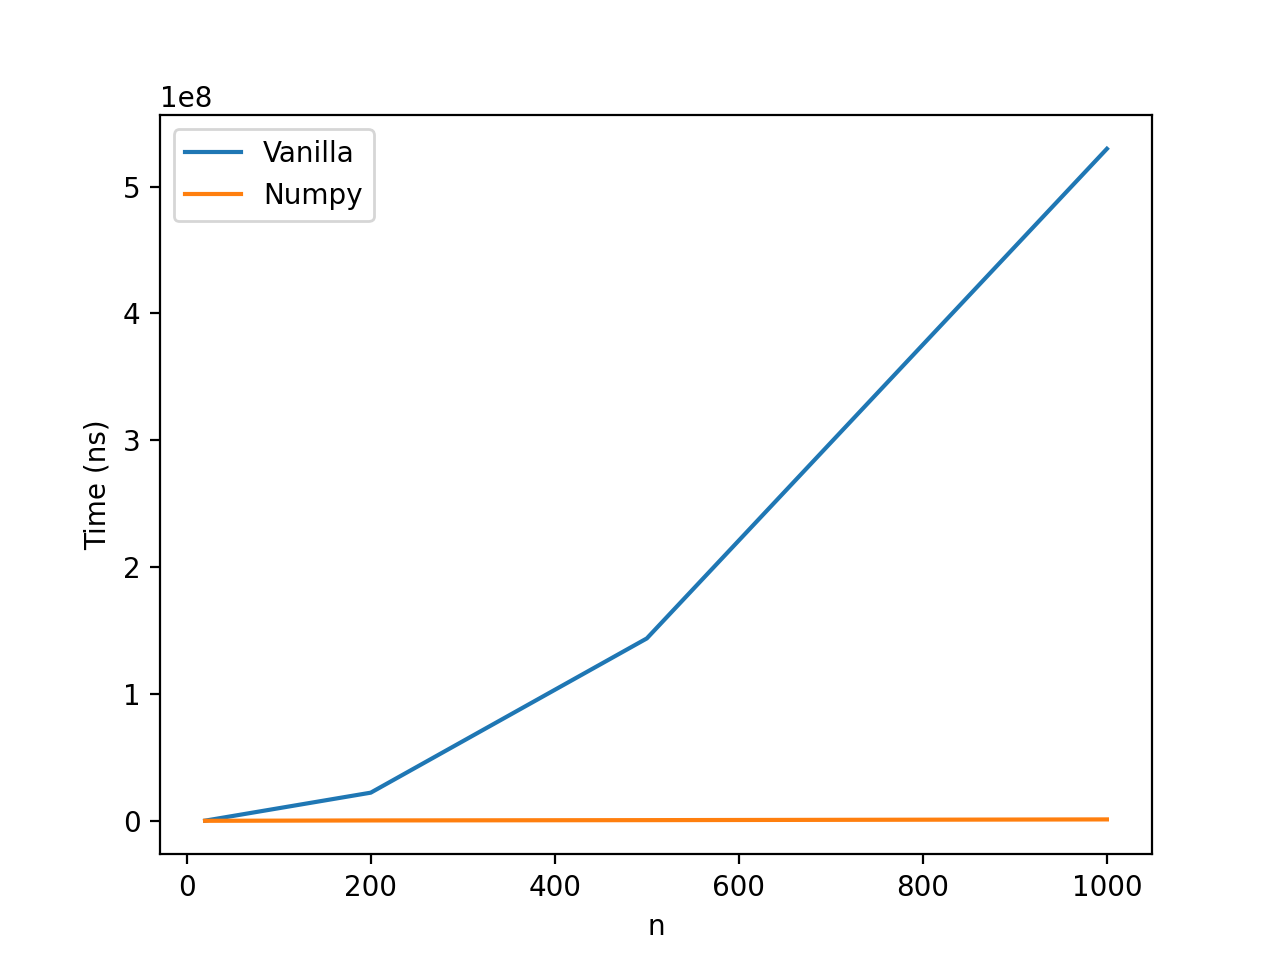
\includegraphics[width=0.5\textwidth]{Figure_1.png}
            \caption{Wall time vs. n (size of vector/matrix) for vanilla and numpy methods.}\label{fig:walltime}
        \end{figure}
        Clearly, Figure \ref{fig:walltime} shows there is a large discrepancy between the vanilla and the numpy methods to get $\nabla_x f(x,y)$. As $n$ increases the computation time for vanilla also increases exponentially, but numpy remains relatively constant.
        This is because numpy performs the operations on the array as a whole while vanilla is running through each individual element in the list one at a time. As a rule of thumb, built-in python functions are better and faster than one you make yourself (especially with for loops).
    \end{enumerate}

    % \subsubsection*{What to Submit:}
    % \begin{itemize}
    %     \item \textbf{Part c:} Difference in wall-clock time for parts a-b
    %     \item \textbf{Part c:} Explanation for above difference (1-2 sentences)
    %     \item \textbf{Code} on Gradescope through coding submission
    % \end{itemize}
\end{aprob}

\newpage
\begin{aprob}
    \points{4} Two random variables $X$ and $Y$ have equal  distributions if their CDFs, $F_X$ and $F_Y$, respectively, are equal, i.e. for all $x$, $ \abs{F_X(x) - F_Y(x)} = 0$. 
    The central limit theorem says that the sum of $k$ independent, zero-mean, variance $1/k$ random variables converges to a (standard) Normal distribution as $k$ tends to infinity.  
    We will study this phenomenon empirically (you will use the Python packages Numpy and Matplotlib).
    Define $Y^{(k)} = \frac{1}{\sqrt{k}} \sum_{i=1}^k B_i$ where each $B_i$ is equal to $-1$ and $1$ with equal probability.
    We know that $\frac{1}{\sqrt{k}} B_i$ is zero-mean and has variance $1/k$.
    \begin{enumerate}
    \item Note that below are descriptions of how the plots are generated. We coded this part up and it is available in zip file. In this problem is meant you will explore matplotlib library, and then explain how solution changes with $k$ in part~\ref{prob:cltcdf:k}.
    \item \label{prob:cltcdf:gaussian} For $i=1,\ldots,n$ let $Z_i \sim \mathcal{N}(0,1)$. If $F(x)$ is the true CDF from which each $Z_i$ is drawn (i.e.,  Gaussian) and $\widehat{F}_n(x) = \frac{1}{n} \sum_{i=1}^n \1\{ Z_i \leq x)$, we will choose $n$ large enough such that, for all $x \in \R$,
    \[
    	\sqrt{\E{\round{\widehat{F}_n(x)-F(x)}^2 }} \leq 0.0025\ ,
    \]
    and plot $\widehat{F}_n(x)$ from $-3$ to $3$.

    \item \label{prob:cltcdf:k} For each $k \in \set{1, 8, 64, 512}$ we will generate $n$ (same as in part D) independent copies $Y^{(k)}$ and plot their empirical CDF on the same plot as part~\ref{prob:cltcdf:gaussian}.
    \end{enumerate}
    Be sure to always label your axes.
    Your plot should look something like the following (up to styling) (Tip: checkout \texttt{seaborn} for instantly better looking plots.)

    \begin{center}
        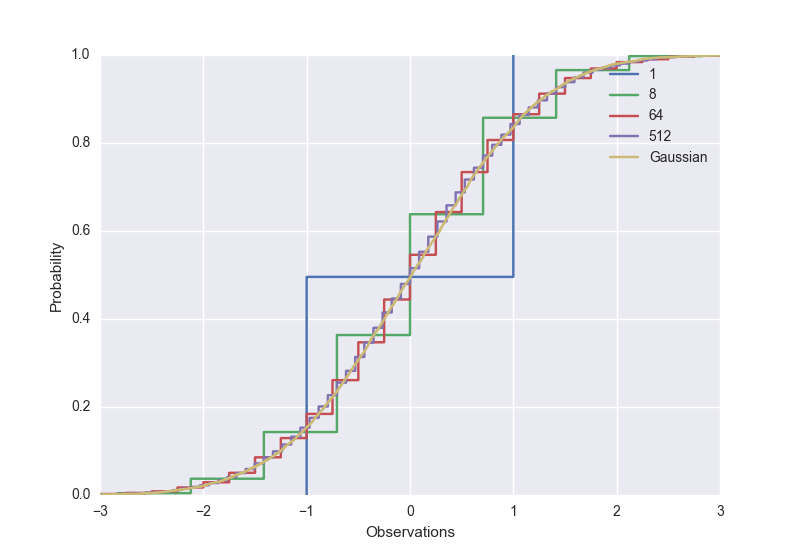
\includegraphics[width=4in]{full.png}
    \end{center}

    \subsubsection*{Solution}
    \begin{itemize}
        \item \textbf{Part~\ref{prob:cltcdf:gaussian}:} Value for $n$  is 40000.
        \item \textbf{Parts a and \ref{prob:cltcdf:k}:} In 1-2 sentences: How does empirical CDF change with $k$?
        \\ The CDF more closely approximates the continuous solution as $k$ increases.
        \item \textbf{Parts~\ref{prob:cltcdf:gaussian} and~\ref{prob:cltcdf:k}:} Plot of $\widehat{F}_n(x) \in [-3, 3]$
        \begin{center}
            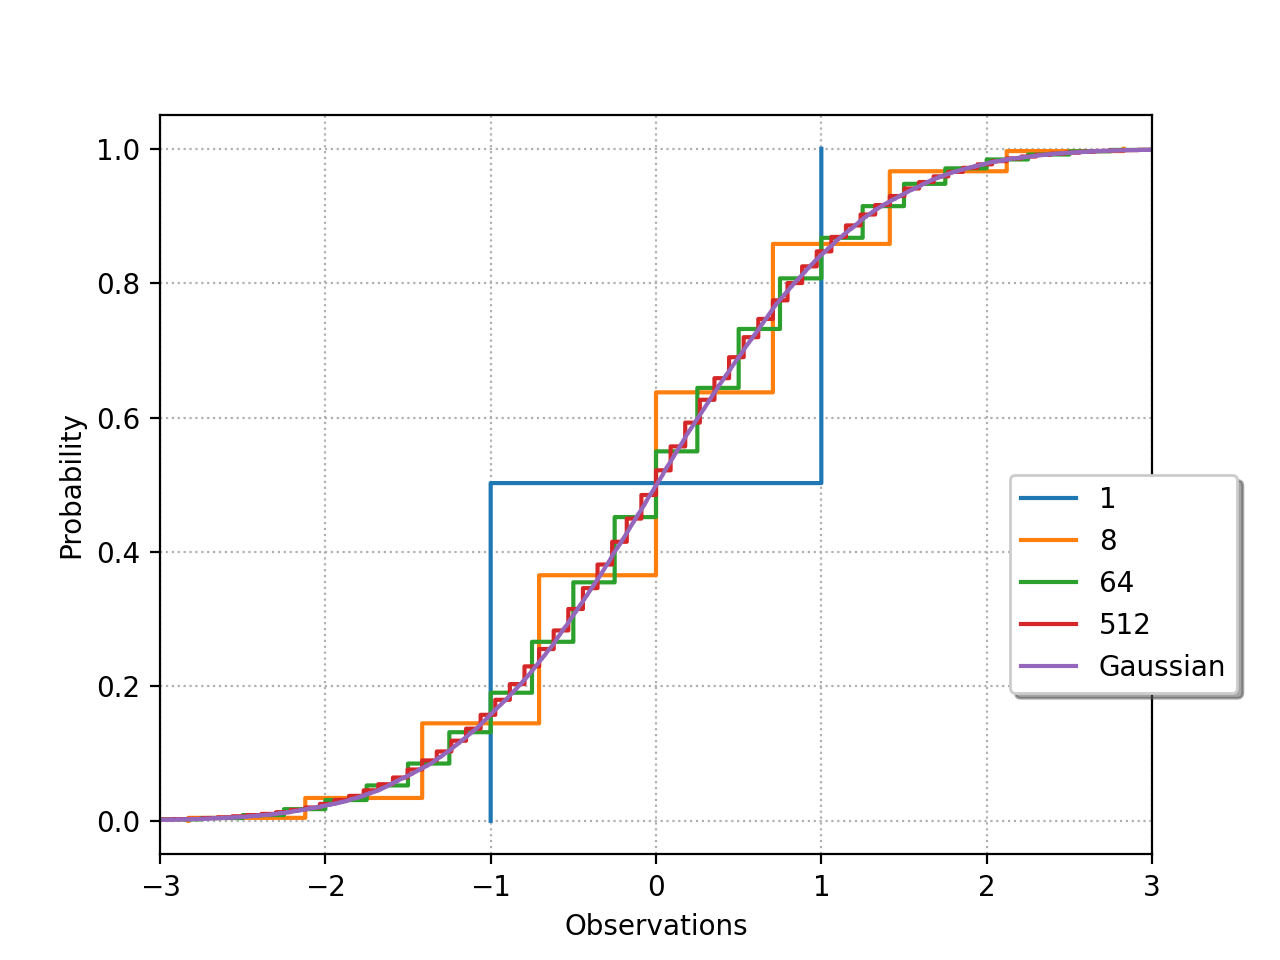
\includegraphics[width=4in]{Figure_2.png}
        \end{center}
    \end{itemize}
\end{aprob}

\end{document}
